\documentclass[a4paper,10pt]{article}
\setlength{\columnsep}{1cm} %space between the columns
\usepackage[utf8]{inputenc}
\usepackage[T1]{fontenc}
\usepackage[english]{babel}
\usepackage[top=2.5cm, bottom=2.5cm, left=2.5cm, right=2.5cm]{geometry}
\usepackage{graphicx} %for the pictures%
\usepackage{hyperref} %to put links in the text%
\usepackage[nottoc,numbib]{tocbibind} %to attribute a number to reference part and in toc
\usepackage[toc,page]{appendix} %to create an appendix part


%%%% HEADER AND FOOT %%%%
\usepackage{fancyhdr}   %libraries for header and foot configuration
\usepackage{lastpage}   %libraries for page count configuration
\pagestyle{fancy}       %call of the page style

%%%% HEADER CONFIGURATION %%%%
\renewcommand\headrulewidth{1pt}    %create a line in the header
\fancyhead[L]{Projektskizzen} 
\fancyhead[R]{Hochschule Ravensburg-Weingarten}
%%%% END OF HEADER CONFIGURATION %%%%

%%%% FOOT CONFIGURATION %%%%
\renewcommand\footrulewidth{1pt}    %create a line in the foot
\fancyfoot[L]{Rémi J. Stéphane S.}
\fancyfoot[C]{\textbf{Page \thepage/\pageref{LastPage}}}
\fancyfoot[R]{October 12, 2023}
%%%% END OF FOOT CONFIGURATION %%%%

%%%% END OF HEADER AND FOOT %%%%


\begin{document}

%%%% FIRST PAGE %%%%
\begin{titlepage}
\pagestyle{empty}
\newcommand{\HRule}{\rule{\linewidth}{0.5mm}}
\center
\textsc{ } \\[3cm]

\includegraphics[scale=0.25]{images/rwu_logo.png} \\[4cm]
\HRule \\[0.4cm]
{ \huge \bfseries Sketch of project: \\[0.15cm] 
 "DockerSec: Cybersecurity Training and Testing Environment" \\[0.4cm]}
\HRule \\[8.6cm]
Authors : 
Rémi JARDRET, Stéphane SIMON\\[0.3cm]
October 12, 2023 \\ [1cm]
\end{titlepage}
%%%% END OF FIRST PAGE %%%%%

%%%% TABLE OF CONTENTS %%%%
\begin{titlepage}
\pagestyle{empty}
\renewcommand{\contentsname}{\center Table of contents\\[2cm]}
\tableofcontents
\end{titlepage}
%%%% END TABLE OF CONTENTS %%%%

%%%% TITLES AND CONTENTS %%%%
\section{Motivations}
The inspiration for this project stemmed from our Linux Administration course at our home institution. In this course, we were tasked with creating an environment comprising a minimum of six virtual machines (VMs) running different Linux distributions. However, this proved to be a labor-intensive process that demanded a lot of hardware resources.\par
On the other side, we also attended classes in cybersecurity, specifically pentesting, where we frequently encountered similar environments. In these classes, we often found ourselves spending around three sessions setting up the environment before we could start our training and pentesting.\par
Following this observation, we concluded that a pre-configured environment with optimized resource utilization would be highly beneficial. Ideally, this environment should be quick and easy to set up. Docker, and in particular Docker Compose, emerged as the perfect solution, offering a streamlined and start-of-the-art solution.


\section{Objectives}
This project is driven by several key objectives, each addressing specific challenges and needs:

\begin{enumerate}
    \item \textbf{Streamlined Environment Setup:} One primary objective is to eliminate the time-consuming and intricate setup of environments for learning and training purposes. The current process of configuring multiple virtual machines (VMs) running different Linux distributions can be arduous, and we aim to simplify this.
    
    \item \textbf{Ease of Deployment:} We also seek to address the challenges related to setting up these environments, making it more user-friendly. The configuration of complex network topologies, including DHCP, DNS, HTTP servers, DMZs, firewalls, and routers, can be daunting for learners and security enthusiasts.
    
    \item \textbf{Resource Optimization:} Resource optimization is a crucial goal. We want to ensure that the environment we provide is efficient in terms of resource utilization, enabling users to run multiple instances simultaneously without overwhelming hardware resources.
\end{enumerate}

Taking these overarching objectives into account, we have defined three specific goals for our project:

\begin{itemize}
    \item \textbf{Facilitating System Administration Learning:} We aim to create an environment where users can explore and understand the intricacies of system administration. This involves gaining insights into the setup and configuration of different components such as "computers," networks, and services. Users can investigate, extend, and experiment with various aspects of system administration.

    \item \textbf{Enhancing Pentesting Training:} Our project seeks to provide a robust platform for pentesting training. This environment will enable users to practice various types of attacks, such as spoofing, scanning, and brute-forcing... Almost all of the Cyber Kill Chain\footnote{https://www.lockheedmartin.com/en-us/capabilities/cyber/cyber-kill-chain.html} can be experimented on this environment.

    \item \textbf{Exploring Docker Capabilities:} This project will serve as an exemplary case among many, enabling learners to delve into more complex Docker setups and explore the full extent of Docker's capabilities.

\end{itemize}

In practical terms, our project aims to deliver an environment consisting of Linux-based machines with integrated features, that will we detail in the next part. This environment will serve as a multifaceted learning platform. Users can look at the configurations, experiment with various scenarios, and advance their knowledge in both system administration and cybersecurity. With the ability to simulate attacks, the project aims to offer an arena for learning and practice.

\newpage

\section{Description}
\subsection{The architecture}
This project aims to create a network architecture using Docker, comprising multiple devices. Within this architecture, two PFsense containers will act as routers and firewalls. Additionally, the setup includes three virtual subnets, numerous servers for services such as DHCP, DNS, and HTTP, and a client computer. The architecture will be divided into several networks, including a DMZ.
\par
From a practical standpoint, we will leverage Docker container images to create our network devices. For instance, we will deploy Docker containers for Linux servers serving as DNS and DHCP servers. To establish the networks, we will employ Macvlan network technology. This will allow us to assign distinct IP addresses and MAC addresses to each container for their respective network interfaces. By using Macvlan, we can connect these containers to separate networks, with PFsense acting as the central router interconnecting these diverse networks.\par

\begin{figure}[bp!]
    \centering
    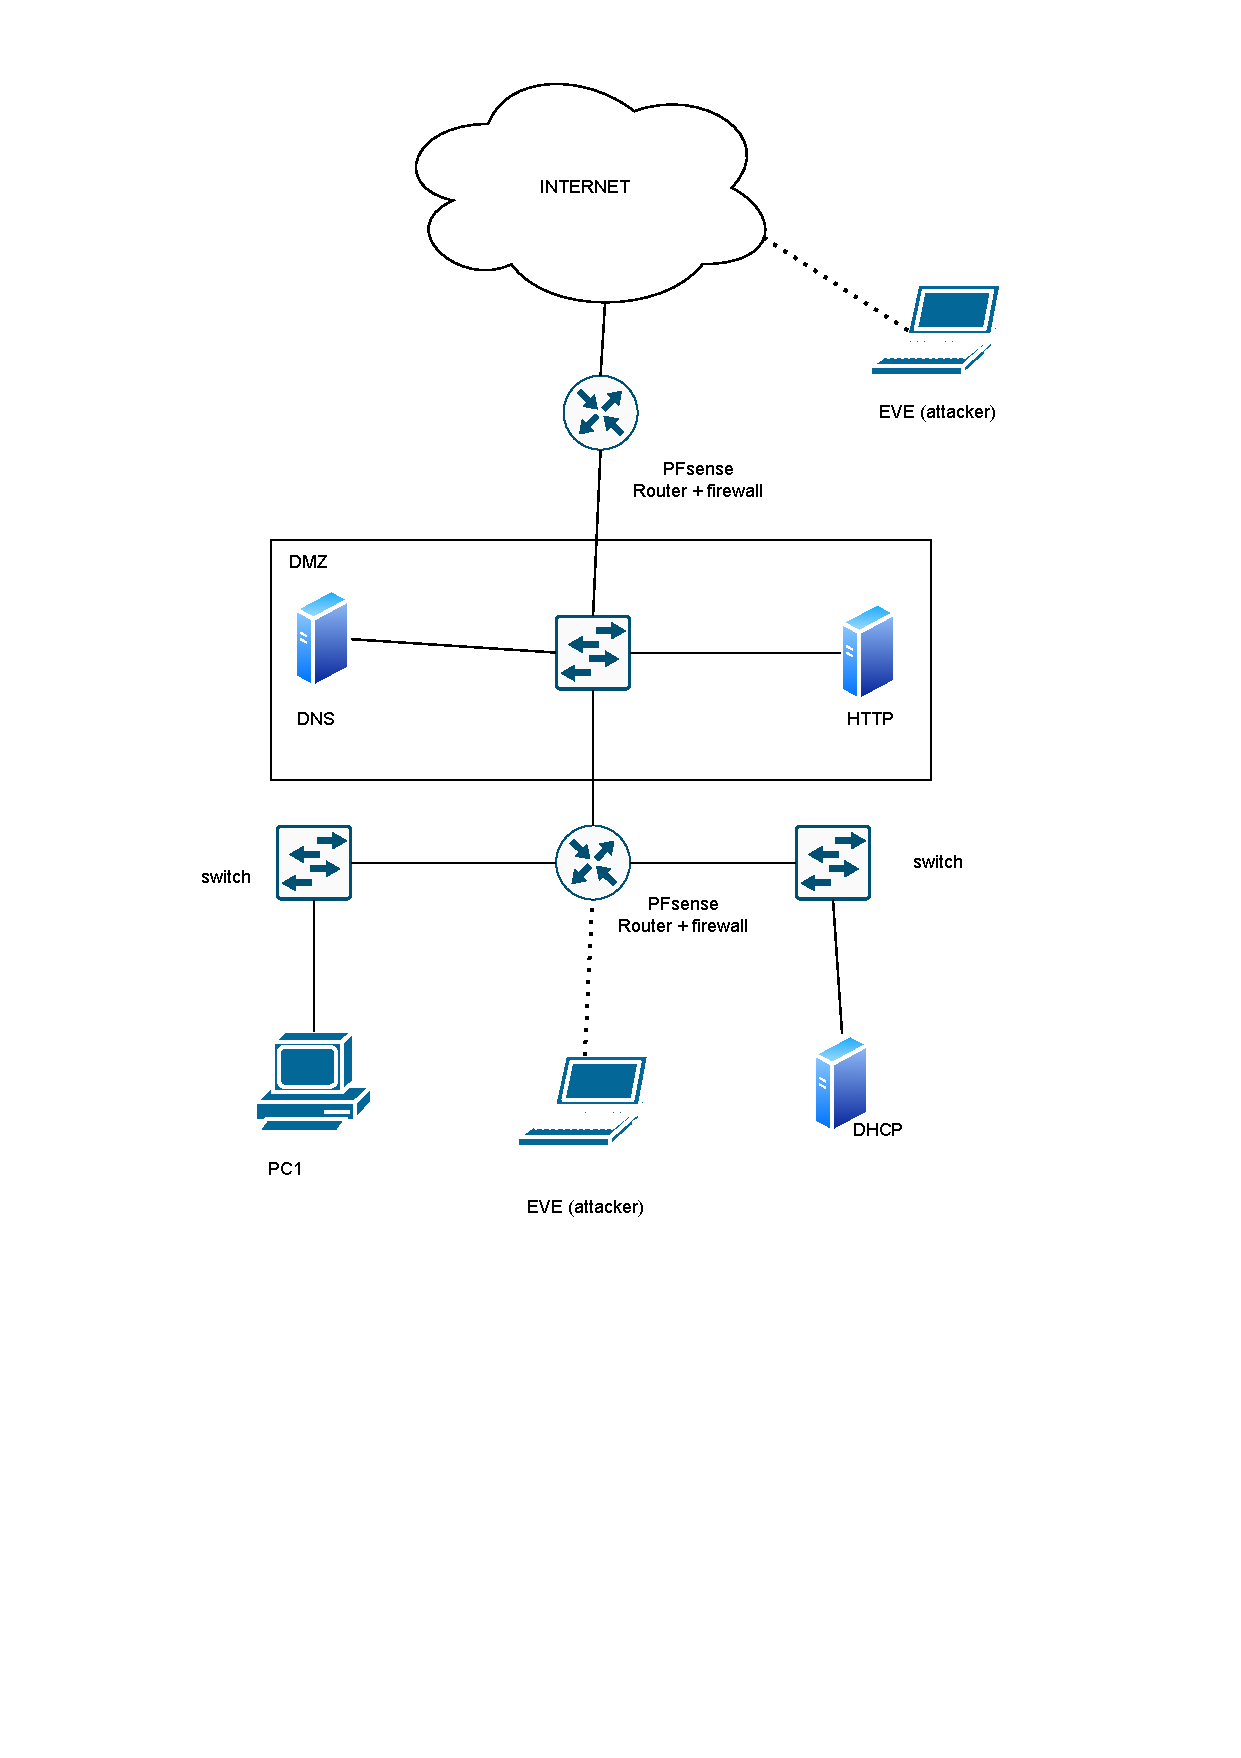
\includegraphics[scale=0.89]{images/architecture_sketch.pdf}
    \caption{Architecture of our project's network}
    \label{fig:1}
\end{figure}

\newpage

\subsection{Eve - The attacker}
Furthermore, we will introduce an attacker, Eve, both inside and outside the network. This will provide opportunities to explore a wide array of attack scenarios and exemplify potential security vulnerabilities.

Eve's role is multifaceted, and we can simulate various real-world cyber threats, including:

\begin{itemize}
    \item \textbf{Spoofing Attacks:} Eve can launch IP and MAC address spoofing attacks to impersonate legitimate devices or alter network traffic.

    \item \textbf{Scanning and Enumeration:} Eve can perform network scanning and enumeration to identify vulnerabilities, open ports, and services on target machines.

    \item \textbf{Brute-Force and Dictionary Attacks:} Eve can attempt login credentials and passwords using brute-force or dictionary attacks on services such as SSH, HTTP, or FTP.

    \item \textbf{DDoS (Distributed Denial of Service):} Eve can launch DDoS attacks to flood network resources, rendering services unavailable.

    \item \textbf{Man-in-the-Middle (MITM) Attacks:} Eve can intercept and manipulate network traffic, potentially eavesdropping on confidential data or injecting malicious content.

    \item \textbf{DNS Poisoning:} Eve can compromise DNS servers to redirect network traffic to malicious websites or domains.

    \item \textbf{Firewall Evasion:} Eve can test the effectiveness of the firewall configurations by attempting to bypass them using various techniques.

    \item \textbf{Exfiltration and Data Theft:} Eve can attempt to steal sensitive data from compromised servers or network traffic.

    \item \textbf{Exploiting Vulnerabilities:} Eve can exploit known vulnerabilities in server software, operating systems, or misconfigured services.

    \item \textbf{Privilege Escalation:} Eve can attempt to elevate privileges on compromised machines to gain deeper access and control.

\end{itemize}

These attack scenarios not only highlight the importance of robust cybersecurity measures but also serve as valuable learning experiences for training in defensive and offensive cybersecurity techniques within a controlled Docker-based environment.

\subsection{Bob - The victim}

Within our network architecture, Bob, also referred to as PC1 in the architectural scheme\ref{fig:1}, assumes the role of the victim computer. To enrich the spectrum of potential attacks and provide a comprehensive learning experience, we will introduce a container like Metasploitable 2.
\par
Metasploitable 2 is a specially designed and intentionally vulnerable version of the Ubuntu Linux operating system. It serves as a valuable tool in pentesting and cybersecurity courses, offering an ideal platform for showcasing a wide range of attack scenarios and techniques. This intentionally vulnerable VM allows learners and security enthusiasts to gain hands-on experience in conducting various security assessments, vulnerability assessments, and penetration testing exercises.


\end{document}
